During the software development activity, there is a major concern in building
programs that can be executed correctly without any failures. Such failures are
the visible consequence of defects hiding in the source code.
Introduced  by developers\footnote{In this research, the term developer
encompasses the roles that are directly involved in the lifecycle of a failure:
analysts, programmers, and maintainers.} due to  human mistakes, some defects
are easily corrected; for example: a simple typo; while others are more
difficult to fix, such as comprehension issues regarding some feature of the
system.

The practice of Software Engineering offers a myriad of testing techniques
attempting to reveal possible existing failures. Once such failures have been
discovered, the following task is to localize and correct the defect that causes
the observable failure. Such a task is called \textit{debugging}.

\section{Context}

Debugging  is the activity whose goal is to detect, locate and correct defects
present in programs. It is an expensive activity which requires developers to
analyze the program's source code as well as its state (stack
trace and memory dumps). In practice, developers use print statements in
code or breakpoints from symbolic debuggers to inspect the state of program
variables in the search for faults. This manual process can be expensive and
ad-hoc~\cite{jones2007}. Recent studies estimate that developers spend half of
their programming time debugging, which approximates to a global cost of 312
billion of dollars a year~\cite{britton2013reversible}.
Several techniques to automate fault localization have been proposed to improve
the debugging process, aiming at reducing effort and time spent
\cite{jones2002visualization,agrawal1995,wotawa2002,zeller2002,renieris2003}.

In particular, some techniques utilize coverage information of code components
such as statements, predicates, def-use associations and call functions to
automate the fault localization process
\cite{jones2002visualization,agrawal1995,wotawa2002}.  Heuristics---based on the
frequency with which code components  are executed in failing and successful
test cases---are used to assign suspiciousness values to statements.  A list of
statements sorted in descending order of suspiciousness is then prepared for the
developer. We call these approaches to fault localization \textit{coverage based
debugging}.

Coverage based debugging information, however, should be presented to the
developer to be useful. An obvious strategy is to list the program's statements
ordered by their values of suspiciousness. Another strategy uses graphical
resources to highlight fault-prone locations.
\textit{SeeSoft}~\cite{eick1992seesoft} is a technique to visualize large
portions of code in which each line of code is displayed as a thin line.
 In the coverage based debugging context, the
suspiciousness value of each line of code defines its hue and brightness
\cite{jones2002visualization}. Figure~\ref{fig:seesoft} presents SeeSoft being
utilized to visualize a faulty program where the more suspicious locations are
colored in bright red. This visualization technique has the advantage of keeping
the code structure (e.g., indentation, line length and blank lines), which
facilitates the understanding of the code.

Nonetheless, current visualization techniques for coverage based debugging lack
contextual information. Suppose that a developer should look for faults in a
large software written in Java as the one described in Figure~\ref{fig:seesoft}.
If she had to choose a package, class and method to initiate her investigation
which one should she start with? If the defect was not found in the first
package, class and method analized, which are the next ones to be investigated?
Such an information is not available in 2D visual metaphors like SeeSoft because
they do not associate suspiciousness with packages, classes and methods---only
with lines of code. In this sense, they fall short of providing a roadmap to
guide the developer in the fault localization process.

\begin{center}
\begin{figure}[h!]
\centerline{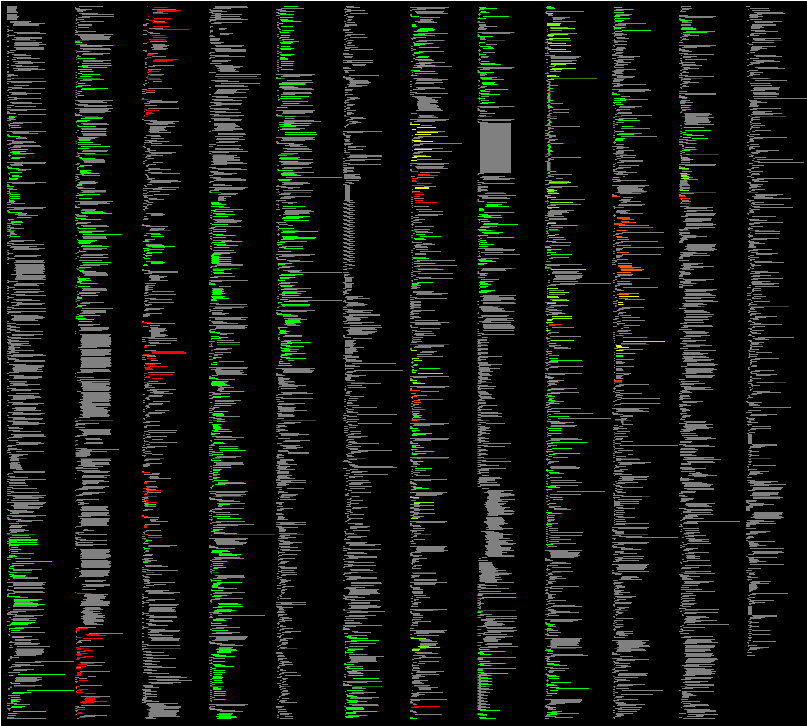
\includegraphics[scale=.7]{figures/eick1992seesoft}}
\caption{SeeSoft utilized to visualize suspicious excerpts of code (obtained from \cite{jones2002visualization}).}\label{fig:seesoft}
\end{figure}
\end{center}

\section{Motivation}

The motivation of this research resides in the observation that current
mechanisms to visualize and inspect debugging information do not provide enough
contextual information to guide the developer towards the fault site. Lists of
suspicious statements and  bidimensional visualization metaphors does not seem
to provide the contextual information required for an effective fault
localization process. Therefore, new visualization metaphors  and mechanisms
that add contextual information are needed to leverage developer's performance
during debugging.

\section{Objectives}

The goal of this work is to develop novel ways to visualize and inspect
debugging information. To achieve such a goal, a new visual metaphor to represent debugging information (e.g., the suspiciousness of code excerpts) is proposed.

In addition, mechanisms to inspect and select debugging information to help the
developer focus her attention onto pieces of code more likely to contain the
fault's site are introduced.

Thus, the overall aim of this research is to improve the developer's experience
in navigating through the information generated by coverage based debugging. A
recent study \cite{parnin2011automated} with developers using coverage based
debugging suggests that additional contextual information might leverage
developers' performance.

This research specific objectives are defined as follows:
\begin{itemize}
 \item Develop  a novel three-dimensional metaphor to represent suspiciousness
 information obtained from coverage based debugging techniques.
 \item Explore how to  display larger program entities,
  namely classes, methods, and their suspiciousness values, in the metaphor.
  \item Embed the new metaphor as a plug-in into a well
  established Integrated Development Environment.
  \item Add contextual information obtained from integration coverage to
  support fault localization \cite{souza13adding}.
  \item Explore new avenues to improve user experience.
  \item Plan and execute an experiment to validate the new metaphor and its
  implementation as a plug-in.
\end{itemize}

\section{Contributions}
%Revisao - Inicio
This research gave origin to several contributions. They are briefly described
in what follows.

\begin{itemize}
    \item A novel three-dimensional metaphor called CodeForest
    (Chapter~\ref{ch:forest}), which aims at representing suspiciousness data
    obtained from coverage based debugging techniques
    (Section~\ref{sec:bg-codecoverage}).

    \item A thorough literature review of 2D and 3D methods to visualize
    software data (Chapter~\ref{ch:related}).

    \item A functional standalone implementation of the CodeForest metaphor
    (Chapter~\ref{ch:forest}), which worked as a sandbox environment to test and
    improve the metaphor.

    \item The CodeForest plug-in (Chapter~\ref{ch:plugin}), embedded into a
    well known Java IDE.

    \item An exploratory experiment (Chapter~\ref{ch:cfexperimentation}) to
    check the adherence of the CodeForest metaphor/plug-in in the activity of
    investigating defects.
\end{itemize}
%Revisao - Fim

\section{Key findings}

In this research, we conducted an exploratory experiment in which the new
metaphor and the features introduced in the plug-in that realizes it were assessed.

We found out that mapping classes into the elements of the new metaphor had a
good reception amongst users. Nevertheless, the positioning of the elements
representing methods according to their score received divergent evaluations and
requires further experiments.

Developers with lower levels of skill in Java are more sympathetic to
investigate the codebase utilizing the new metaphor virtual environment. They do
utilize contextual information (also known as ``roadmap'') to filter the
elements of the metaphor, but the primary investigation happens in the virtual
environment.

More experienced users prefer to solely use the roadmap as an investigation
guide, and utilize the filtering tools to check the remaining elements. This
way, they are able to assess which elements of the codebase should be inspected
and move on directly to the source code.

\section{Organization}

This chapter presented the context, motivation and objectives of our research,
whose main objective is to develop novel ways to select, visualize, and inspect
debugging information.

The remainder of this document is organized as follows.
\begin{itemize}
  \item Chapter~\ref{ch:background} presents the necessary background in
  software testing, coverage based debugging, and software visualization.
  \item Chapter~\ref{ch:related} examines the related work.
  \item Chapter~\ref{ch:forest} presents a new metaphor for visualizing coverage
  based debug information, its design rationale, and a prototype software,
  developed to test the feasibility of our ideas.
  \item Chapter~\ref{ch:plugin} contains the details required to turn a
  prototype into a complete tool, embedded in the Eclipse Platform.
  \item Chapter~\ref{ch:cfexperimentation} describes an experiment in which the
  use of the Eclipse plug-in is assessed.
  \item Chapter~\ref{ch:conclusions} draws conclusions and lists possible
  extensions to this research.
\end{itemize}